\documentclass[12pt,a4paper]{article}

\usepackage[utf8]{inputenc}
\usepackage[italian]{babel}
\usepackage{amsmath}
\usepackage{amsfonts}
\usepackage{amssymb}
\usepackage{graphicx}
\usepackage{booktabs}
\usepackage{float}
\usepackage[margin=1.95cm]{geometry}
\usepackage{fancyhdr}
\usepackage{siunitx}
\usepackage{xcolor}
\definecolor{darkblue}{RGB}{0,51,102}
\usepackage{hyperref}
\hypersetup{colorlinks=true, linkcolor=darkblue, urlcolor=darkblue, citecolor=darkblue}
\usepackage{caption}
\usepackage{subcaption}
\usepackage{microtype}
\usepackage{setspace}
\usepackage{needspace}
\usepackage{placeins}
\setstretch{0.97}

\pagestyle{fancy}
\fancyhf{}
\rhead{Gruppo 7}
\lhead{Risk Management 2025/2026}
\cfoot{\thepage}
\graphicspath{{latex_report/figures/}{latex_report/copertina/}{figures/}{./}}
\setlength{\parindent}{0pt}
\setlength{\parskip}{0.38em}
\setlength{\textfloatsep}{6pt plus 2pt minus 2pt}
\setlength{\abovecaptionskip}{4pt}
\setlength{\belowcaptionskip}{2pt}

\newcommand{\VaR}{\ensuremath{\mathrm{VaR}}}
\newcommand{\USD}{\ensuremath{\,\$}}

\begin{document}

\begin{titlepage}
\centering

\includegraphics[width=0.55\textwidth]{IMG_2018.jpeg}\\[0.5cm]
\vspace*{1cm}
{\Huge\bfseries Progetto di Risk Management\\[0.3cm]}
{\Large\bfseries Analisi di Rendimenti, Volatilità e VaR\\[0.8cm]}
{\LARGE Quantitative Finance 2025/2026\\[0.8cm]}
{\large Docente: Aldo Nassigh e Michele Bonollo\\[1cm]}
{\large Maggio 2026\\[1.5cm]}
{\Large\bfseries Gruppo 7\\[0.5cm]}
{\large Edoardo Ercelli - Luca Galli - Francesco Impenati - Francesco Mazzini\\[1cm]}
\vspace*{0.5cm}
\end{titlepage}

\tableofcontents
\newpage

% =============================================================================
\section{Punto 1: Selezione titoli, prezzi e rendimenti}
% =============================================================================

\subsection*{Scelte metodologiche}

La consegna impone sette equity in dollari: selezioniamo solo titoli US quotati in USD (suffissi Bloomberg \texttt{US}/\texttt{UN}) per non mescolare valute. Un errore di valuta renderebbe i rendimenti non comparabili e gonfierebbe o sgonfierebbe artificialmente volatilità e correlazioni.

Misuriamo le variazioni con \textbf{log-rendimenti} $g_{i,t}=\ln(P_{i,t}/P_{i,t-1})$ anziché rendimenti semplici $R_t=P_t/P_{t-1}-1$ perché: (i) sono additivi nel tempo, requisito per orizzonti $H>1$ e per sommare shock nel \VaR; (ii) sono la variabile standard su cui si costruiscono GARCH e \VaR\ gaussiano; (iii) per variazioni giornaliere moderate approssimano meglio la simmetria. \textbf{Conseguenza pratica:} se usassimo rendimenti semplici, la conversione in perdita monetaria e il confronto tra metodi perderebbero coerenza interna; i rendimenti semplici restano solo per interpretare il total return del portafoglio (Punto~4.a), dove l'investitore ragiona in percentuale sul capitale.

\textbf{Selezione settoriale.} Evitiamo sette titoli dello stesso settore: correlazioni quasi unitarie renderebbero illusoria la diversificazione al Punto~4.d. Il pannello è \textbf{Danaher} (DHR, life science/diagnostica), \textbf{Edwards Lifesciences} (EW, medical devices), \textbf{The Hartford} (HIG, assicurazioni), \textbf{Nasdaq} (NDAQ, exchange), \textbf{Palo Alto Networks} (PANW, cybersecurity), \textbf{Teledyne} (TDY, aerospace/defense), \textbf{Vertex} (VRTX, biotech): large cap US liquide. \textbf{Vantaggio:} esposizione a fattori di rischio diversi (regolazione, tassi, ciclo tech, sanitario). \textbf{Limite:} restano tutti equity US; in fasi di sell-off generalizzato le correlazioni tendono a salire comunque, come vedremo.

Il campione comune ($1131$ giorni, 19/07/2021--17/11/2025) include il rialzo post-pandemia, il ribasso del 2022 e la ripresa successiva: la volatilità stimata non è ``tranquilla'' per costruzione, il che rende più credibile il test ``vol costante?'' del Punto~4.e.

\subsection*{Lettura della Figura~\ref{fig:p1_prices}}

I prezzi sono normalizzati a $100$ alla prima data comune: confronto di traiettorie relative senza distorsione da prezzi assoluti. Si osservano cali sincronizzati (2022) e recuperi differenziati: PANW e VRTX oscillano di più; HIG e NDAQ più stabili. La figura non entra nelle formule di \VaR, ma giustifica perché un solo numero di volatilità statica (Punto~2) può essere insufficiente e perché le correlazioni vanno stimate esplicitamente.

\begin{figure}[H]
\centering
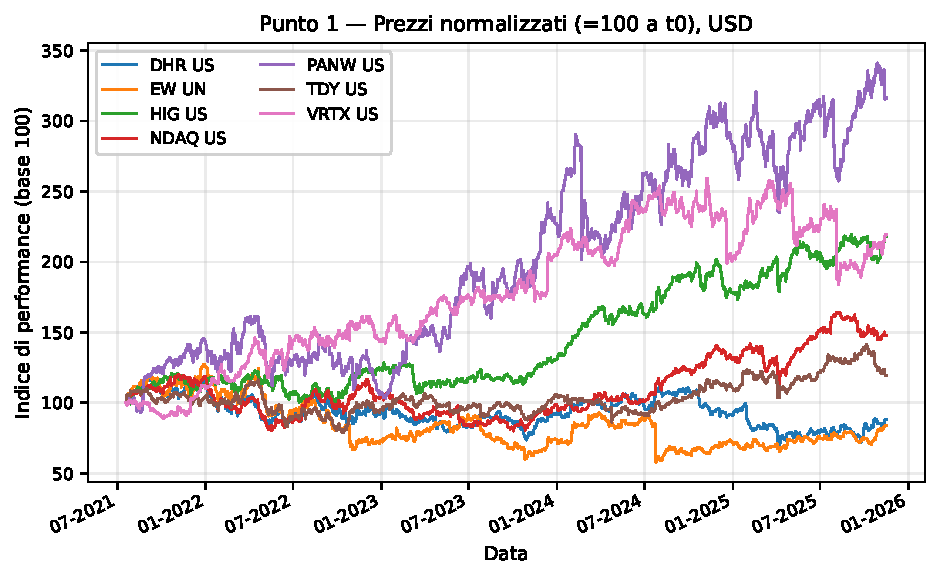
\includegraphics[width=0.88\textwidth]{p1_prices_normalized_report.pdf}
\caption{Prezzi normalizzati (base 100, USD).}
\label{fig:p1_prices}
\end{figure}

% =============================================================================
\section{Punto 2: Statistiche, volatilità e correlazioni}
% =============================================================================

\subsection*{Scelte metodologiche}

\textbf{Normalità e statistiche.} Calcoliamo media, $\hat\sigma$, skewness, kurtosi e Jarque--Bera su $H_0$: normalità. Il rigetto su tutti i titoli ($p\ll 0{,}01$) segnala \textbf{code spesse} (kurtosi $>3$) e possibile \textbf{asimmetria} (skewness $\neq 0$). \textbf{Conseguenza:} il \VaR\ gaussiano sottostima o sovrastima le perdite estreme a seconda del segno delle code; resta utile come \emph{benchmark} confrontabile e come base del MC, non come misura ``vera'' del rischio. Da qui: innovazioni Student-$t$ nei GARCH (più massa nelle code) e \VaR\ storico affiancato nei Punti~3--4. \textbf{Alternativa scartata:} usare solo modelli GARCH per il \VaR\ giornaliero avrebbe introdotto vol condizionata diversa dal parametrico statico e reso opaco il confronto tra metodi.

\textbf{Annualizzazione.} $\hat\sigma_{\mathrm{ann}}=\hat\sigma_{\mathrm{giorno}}\sqrt{252}$: radice del tempo sotto ipotesi di rendimenti i.i.d.\ giornalieri (approssimazione standard). La vol \textbf{statica} è su tutto il campione (un solo numero, stabile ma lento ad aggiornarsi). Le vol \textbf{rolling} su $21$g ($\approx$1M), $63$g (3M, solo diagnostica) e $252$g (1Y) misurano il regime corrente: \textbf{vantaggio} sensibilità agli shock recenti; \textbf{svantaggio} maggiore rumore e valori mancanti all'inizio delle serie finché la finestra non si riempie.

\textbf{EWMA e due valori di $\lambda$.} L'EWMA aggiorna la varianza con $\sigma_t^2=\lambda\sigma_{t-1}^2+(1-\lambda)r_t^2$. Con $\lambda=0{,}94$ (standard RiskMetrics per dati \textbf{giornalieri}) il peso sullo shock di oggi è solo il 6\%, mentre il 94\% viene dalla vol di ieri: la serie è liscia e adatta a captare \textbf{volatility clustering} (periodi di calma e di stress raggruppati, coerenti con l'\textbf{effetto ARCH} di autocorrelazione in $g_t^2$). Se $\lambda$ fosse 0,80 la vol reagirebbe troppo ai singoli giorni (rumore); se fosse 0,99 sarebbe quasi statica e perderebbe utilità di monitoraggio. Inizializziamo la ricorsione sui primi $30$ giorni perché all'avvio del campione non esiste una ``vol di ieri'' affidabile. Sul \textbf{portafoglio} (Punto~4.e) usiamo $\lambda\approx 0{,}909$, ottenuto dalla relazione $\lambda=1-2/(h+1)$ con $h=21$ giorni: equivale a un orizzonte di circa un mese di negoziazione, più reattivo del 0,94 e allineato alla vol rolling 21g del Punto~4.b. \textbf{Implicazione:} due $\lambda$ non sono un errore, ma due orizzonti decisionali (rischio strutturale giornaliero vs.\ rischio del ultimo mese sul portafoglio).

\textbf{GARCH e EGARCH.} Il modello GARCH$(1,1)$ scrive $\sigma_t^2=\omega+\alpha\varepsilon_{t-1}^2+\beta\sigma_{t-1}^2$ con innovazioni $\varepsilon_t$ Student-$t$. Il coefficiente $\alpha$ misura quanto uno shock al quadrato ieri sposta la vol odierna (\textbf{effetto ARCH}: volatilità che si accende dopo movimenti ampi); $\beta$ misura la persistenza (vol alta che resta alta). Se $\alpha+\beta$ è vicino a 1, gli shock si dissipano lentamente (\textbf{volatility clustering}). \textbf{Perché Student-$t$?} Jarque--Bera rigetta la normalità: le code empiriche sono più spesse; il $t$ evita di sottostimare estremi nella dinamica della vol. Se $\hat\beta\approx 0$ (stima al confine, vol quasi costante nel GARCH) passiamo a \textbf{EGARCH}$(1,1,1)$ su $\ln\sigma_t^2$: può modellare l'\textbf{effetto leva} (bad news che alzano la vol più delle good news simmetriche, tipico delle equity) e non impone $\sigma_t^2>0$ tramite vincoli su $\omega,\alpha,\beta$ come nel GARCH. \textbf{Implicazione pratica:} GARCH/EGARCH descrivono \emph{come} evolve il rischio nel tempo; il \VaR\ parametrico del Punto~3 usa invece una $\hat\sigma$ media sul campione, così confrontiamo tre metodi sulla stessa ipotesi statica e usiamo GARCH solo per diagnosticare se quella media è fuorviante (Punti~2 e~4.e).

\textbf{Correlazioni e livello $\alpha=5\%$ sul test.} Pearson \emph{listwise} ($n=1130$): eliminiamo date con un solo missing, così $\hat{\boldsymbol\Sigma}$ è definita positiva e coerente col \VaR\ multivariato. Test $H_0\colon\rho_{ij}=0$ con statistica $t$ a due code; rifiutiamo se $p<5\%$. \textbf{Perché 5\% e non 1\% o 10\%?} Al 1\% segnaleremmo meno coppie (più errori Tipo II: ignorare correlazioni vere); al 10\% troveremmo quasi tutto significativo anche con $\hat\rho$ economicamente piccolo (più errori Tipo I). Il 5\% è il compromesso standard nei report di rischio. Con $n$ grande, anche $\hat\rho\approx 0{,}15$ può risultare significativo: per questo nel Punto~4.d leggiamo anche la \emph{magnitudine}, non solo il $p$-value. \textbf{Spearman scartato:} misura monotonia, non lineare; il \VaR\ var-cov richiede covarianze (Pearson).

\subsection*{Volatilità (Figure~\ref{fig:p2_volcompare}--\ref{fig:p2_vol_overlay})}

La Fig.~\ref{fig:p2_volcompare}: blu = vol statica; arancione = rolling 1Y ultima data. Divergenze su VRTX, DHR, PANW: il lungo periodo non descrive il regime attuale; un risk manager che usasse solo la statica \emph{sottostimerebbe} o \emph{sovrastimerebbe} il rischio odierno. PANW supera il $38\%$ annualizzato sull'ultimo 1Y rolling.

La Fig.~\ref{fig:p2_vol_overlay}: rolling 1Y, EWMA ($\lambda=0{,}94$), GARCH-$t$. Quando GARCH ed EWMA salgono insieme (2022) c'è vol condizionata oltre la media mobile. Se solo la rolling sale e GARCH resta piatto, lo shock potrebbe essere stato isolato; se tutte e tre salgono, il regime è strutturalmente più rischioso.

\begin{figure}[H]
\centering
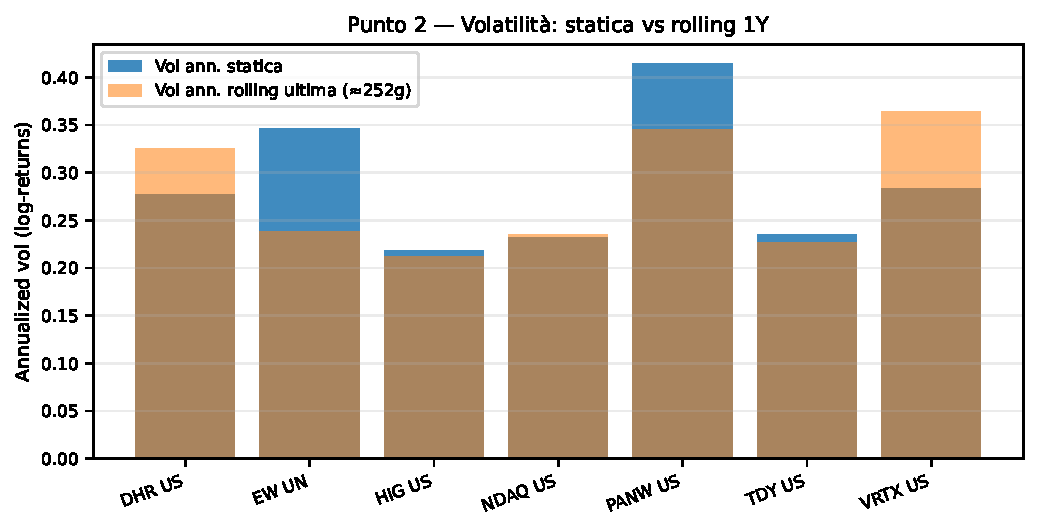
\includegraphics[width=0.86\textwidth]{p2_vol_summary_static_vs_roll1y.pdf}
\caption{Volatilità statica vs.\ rolling 1Y (ultima osservazione).}
\label{fig:p2_volcompare}
\end{figure}

\begin{figure}[H]
\centering
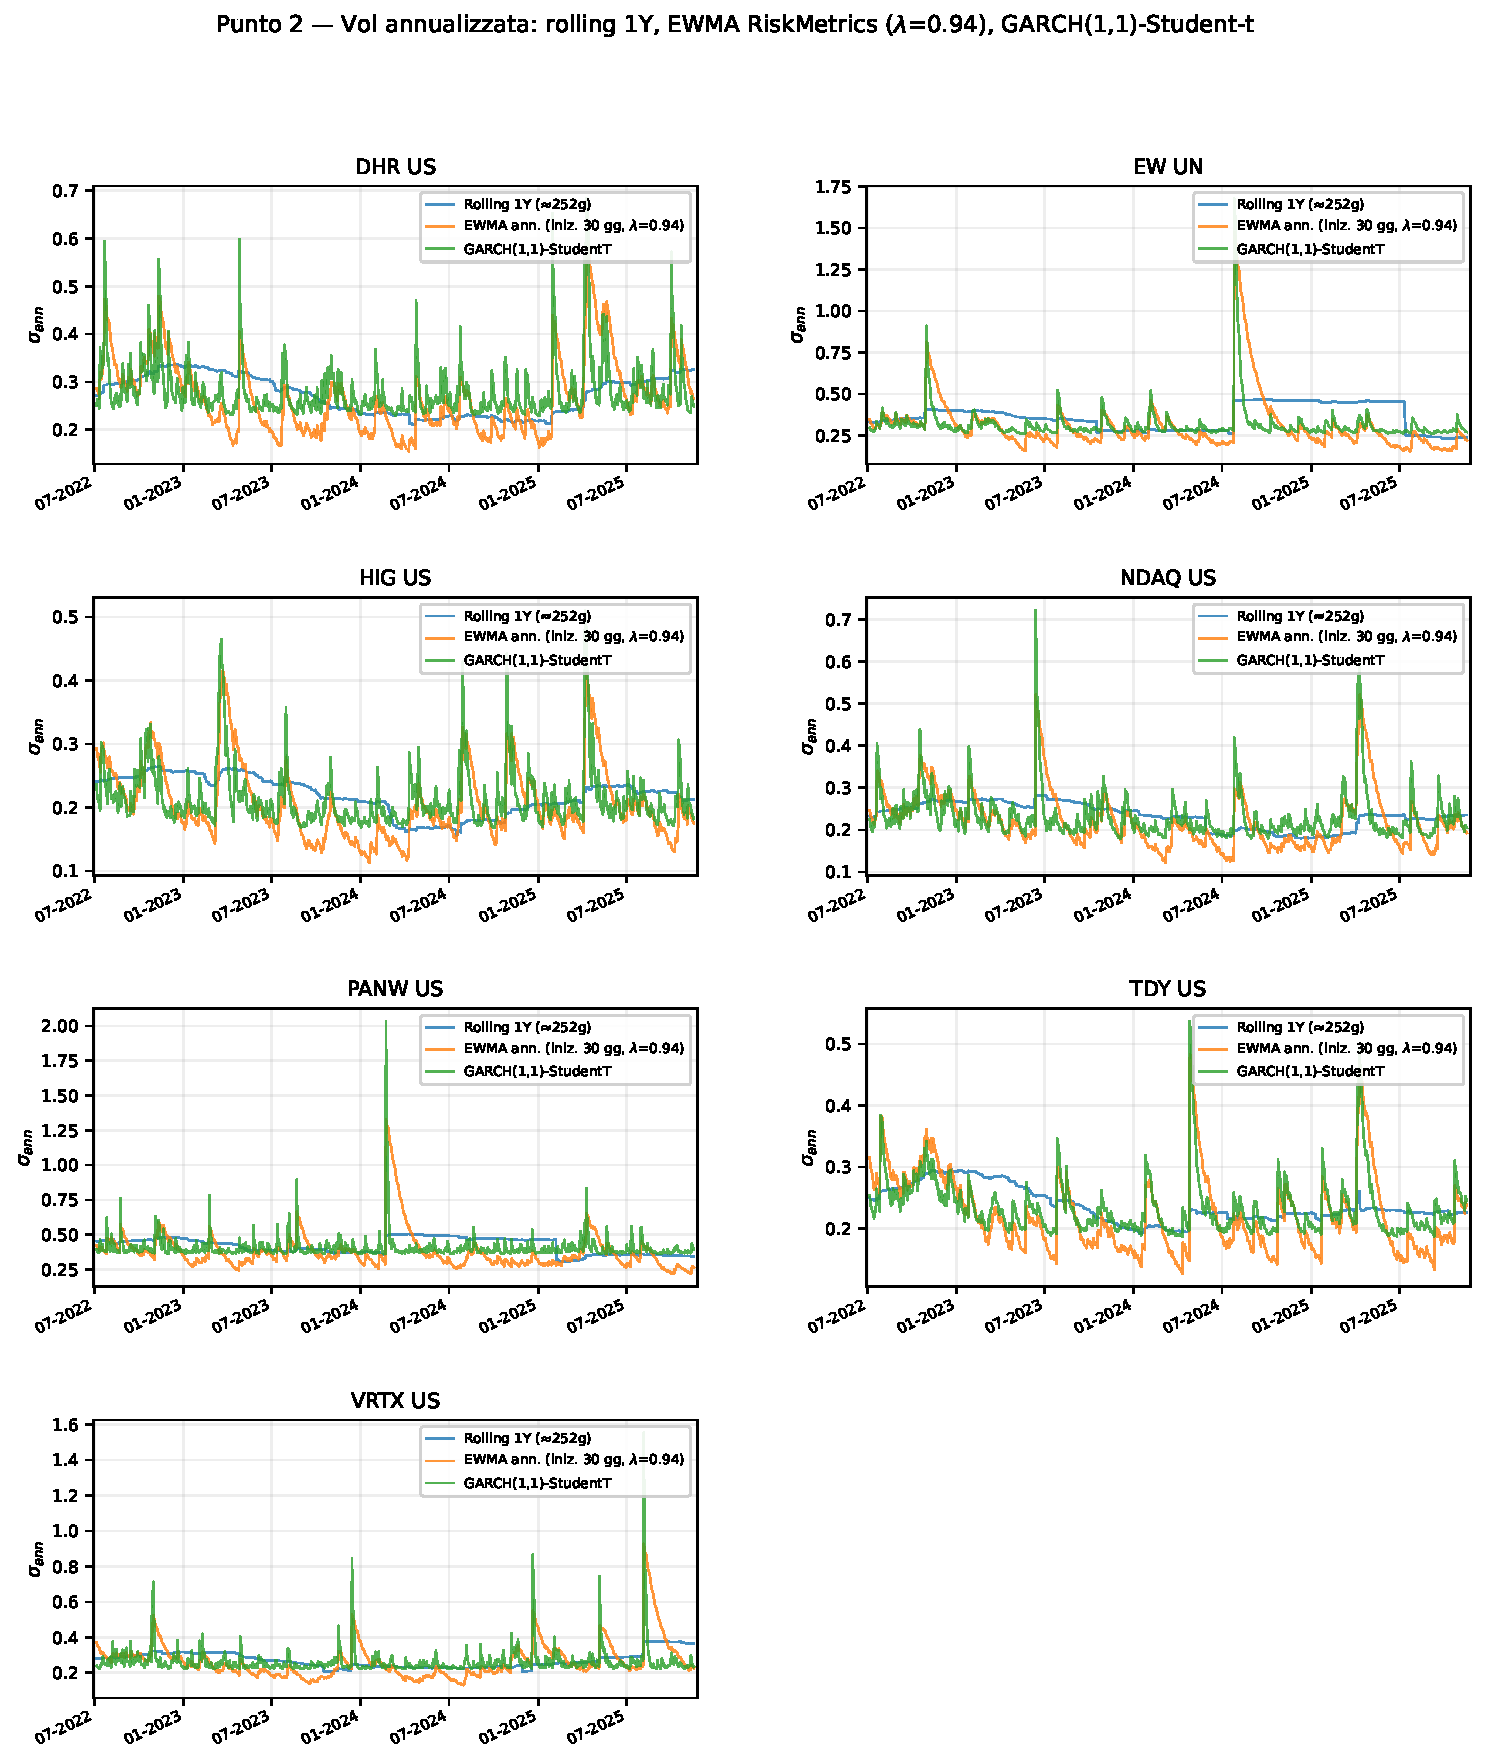
\includegraphics[width=0.88\textwidth]{p2_vol_overlay_roll_ewma_garch_panels.pdf}
\caption{Rolling 1Y, EWMA ($\lambda=0{,}94$) e GARCH$(1,1)$-$t$ per titolo.}
\label{fig:p2_vol_overlay}
\end{figure}

\subsection*{Correlazioni (Figura~\ref{fig:p2_corrpair})}

Tutte le $21$ coppie significative al $5\%$: nessun hedge lineare negativo. $\hat\rho_{ij}$ positivi e moderati (non un portafoglio ``quasi monocollina'', ma nemmeno indipendente). La mappa $-\log_{10}(p)$ evidenzia uniforme significatività statistica: \textbf{conseguenza} per il portafoglio, ignorare le correlazioni (matrice diagonale) \emph{sottostimerebbe} il rischio sistematico condiviso.

\begin{figure}[H]
\centering
\begin{subfigure}[t]{0.49\textwidth}
\centering
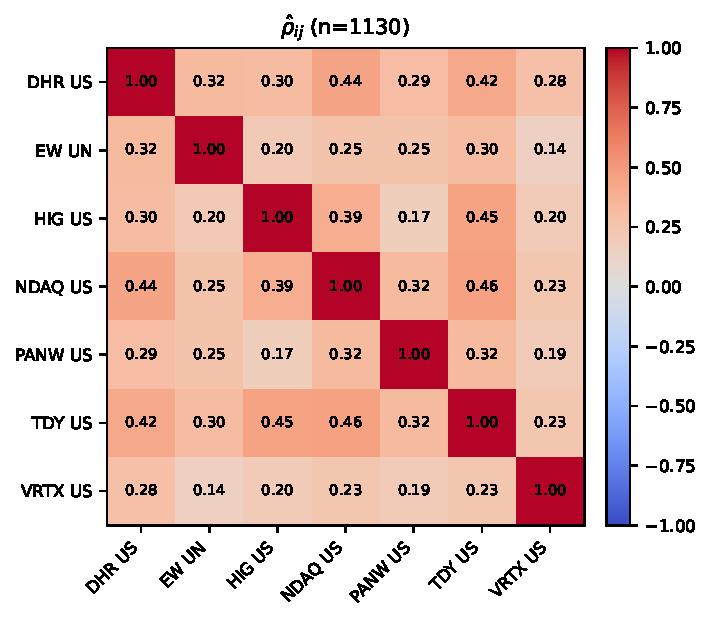
\includegraphics[width=\textwidth]{p2_corr_heatmap.pdf}
\caption{$\hat\rho_{ij}$.}
\end{subfigure}\hfill
\begin{subfigure}[t]{0.49\textwidth}
\centering
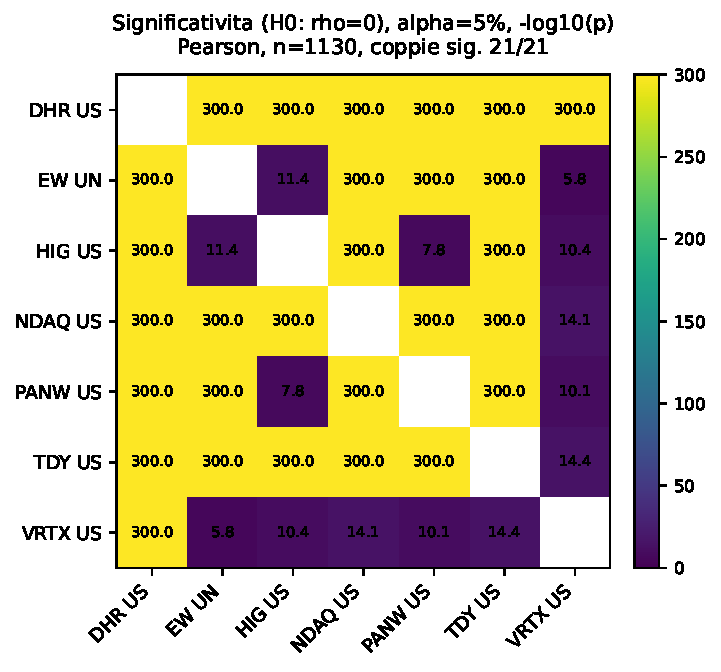
\includegraphics[width=\textwidth]{p2_corr_pvalues_heatmap.pdf}
\caption{$-\log_{10}(p)$, test al $5\%$.}
\end{subfigure}
\caption{Correlazioni di Pearson e significatività ($n=1130$).}
\label{fig:p2_corrpair}
\end{figure}

% =============================================================================
\section{Punto 3: Value-at-Risk per singolo titolo}
% =============================================================================

\subsection*{Scelte metodologiche}

\textbf{Livello di confidenza e orizzonte.} $\alpha=5\%$ sulla coda sinistra dei rendimenti: \VaR\ al 95\% nel linguaggio del corso (probabilità del 5\% di perdita giornaliera peggiore del quantile, sotto le ipotesi del metodo). \textbf{Perché non 1\%?} Un \VaR\ più estremo sarebbe più conservativo ma meno stabile (pochi dati nella coda). \textbf{Perché non 10\%?} Sarebbe troppo permissivo per un report di rischio giornaliero. $H=1$ giorno rispetta la consegna; per $H>5$ la gaussiana i.i.d.\ con scaling $\sqrt{H}$ ignora autocorrelazione e effetti di aggregazione non lineari.

\textbf{Capitale e interpretazione.} $M=100\,000\USD$ \emph{per titolo}: ogni barra del grafico misura il rischio su un capitale dedicato a un solo titolo. \textbf{Conseguenza:} non sommare mentalmente quelle barre per ottenere il \VaR\ di portafoglio (errore fatto esplicito al Punto~4.c).

\textbf{Monte Carlo.} $N=50\,000$ simulazioni: l'errore standard sul quantile simulato diventa trascurabile rispetto alle differenze tra metodi; con $N=5\,000$ vedremmo più rumore senza cambiare le conclusioni. Seed fisso: riproducibilità in sede di consegna. Il MC campiona dalla stessa $\mathcal{N}(\hat\mu,\hat\sigma^2)$ del parametrico: \textbf{deve} coincidere se il codice è corretto; la divergenza parametrico/MC segnalerebbe un bug, non un insight economico.

\textbf{Perché non GBM sui prezzi e perché non vol GARCH nel \VaR.} GBM simulerebbe prezzi positivi con drift e vol; a un giorno, sotto gaussianità dei log-rendimenti, è equivalente a campionare $g_t$, ma a orizzonti più lunghi le ipotesi divergono. Usare $\sigma_t^{\mathrm{GARCH}}$ nel \VaR\ significherebbe rispondere alla domanda ``quanto perdo oggi se la vol condizionata odierna è alta'', diversa da ``quanto perdo usando la dispersione media del campione''. Abbiamo scelto la seconda per allineare parametrico, storico e MC.

\textbf{Storico e quantile.} $\VaR_g=-Q_{5\%}(g)$ empirico, interpolazione lineare tra ordinate adiacenti: nessuna ipotesi sulla forma della distribuzione. \textbf{Vantaggio:} cattura asimmetria e code reali. \textbf{Svantaggio:} dipende dal campione (se non ci sono crisi nel periodo, sottostima le code).

Perdita USD su posizione long: $\VaR_{\mathrm{USD}}\approx M(1-e^{-\VaR_g})$. Per $|g|$ piccoli si approssima a $M\cdot\VaR_g$; per perdite più grandi la formula esponenziale evita sottostima.

\textbf{Backtest out-of-sample.} Stima \VaR\ sulla prima metà del campione, violazioni sulla seconda. Target: frequenza violazioni $\approx 5\%$. \textbf{Se $\gg 5\%$:} il modello è troppo ottimistico (sottostima il rischio). \textbf{Se $\ll 5\%$:} modello troppo conservativo o periodo di calma nella seconda metà. Non è test di Kupiec formale, ma controllo direzionale richiesto da uno stile report direzionale.

\subsection*{Risultati (Figura~\ref{fig:p3_var})}

Parametrico $\approx$ MC: validazione implementativa. Storico più basso su EW, VRTX: nel campione le code empiriche sono meno spesse della gaussiana con la stessa $\hat\sigma$ (il \VaR\ storico non ``dà per scontata'' la normalità). PANW massimo ($\approx\$4{,}1$k), coerente con vol Punto~2: il titolo più volatile è anche quello con maggiore perdita potenziale a un giorno. Pannello OOS: eventuali scostamenti dal 5\% invitano a non fidarsi ciecamente del solo parametrico in quei nomi.

\begin{table}[H]
\centering
\footnotesize
\caption{\VaR\ 1g, $\alpha=5\%$, $M=100\,000\USD$ per titolo.}
\begin{tabular}{lrrr}
\toprule
\textbf{Ticker} & \textbf{Param.} & \textbf{Stor.} & \textbf{MC} \\
\midrule
DHR & 2{,}843 & 2{,}679 & 2{,}851 \\
EW  & 3{,}540 & 2{,}694 & 3{,}530 \\
HIG & 2{,}172 & 2{,}175 & 2{,}178 \\
NDAQ& 2{,}345 & 2{,}267 & 2{,}333 \\
PANW& 4{,}100 & 3{,}727 & 4{,}088 \\
TDY & 2{,}389 & 2{,}285 & 2{,}403 \\
VRTX& 2{,}830 & 2{,}326 & 2{,}818 \\
\bottomrule
\end{tabular}
\end{table}

\begin{figure}[H]
\centering
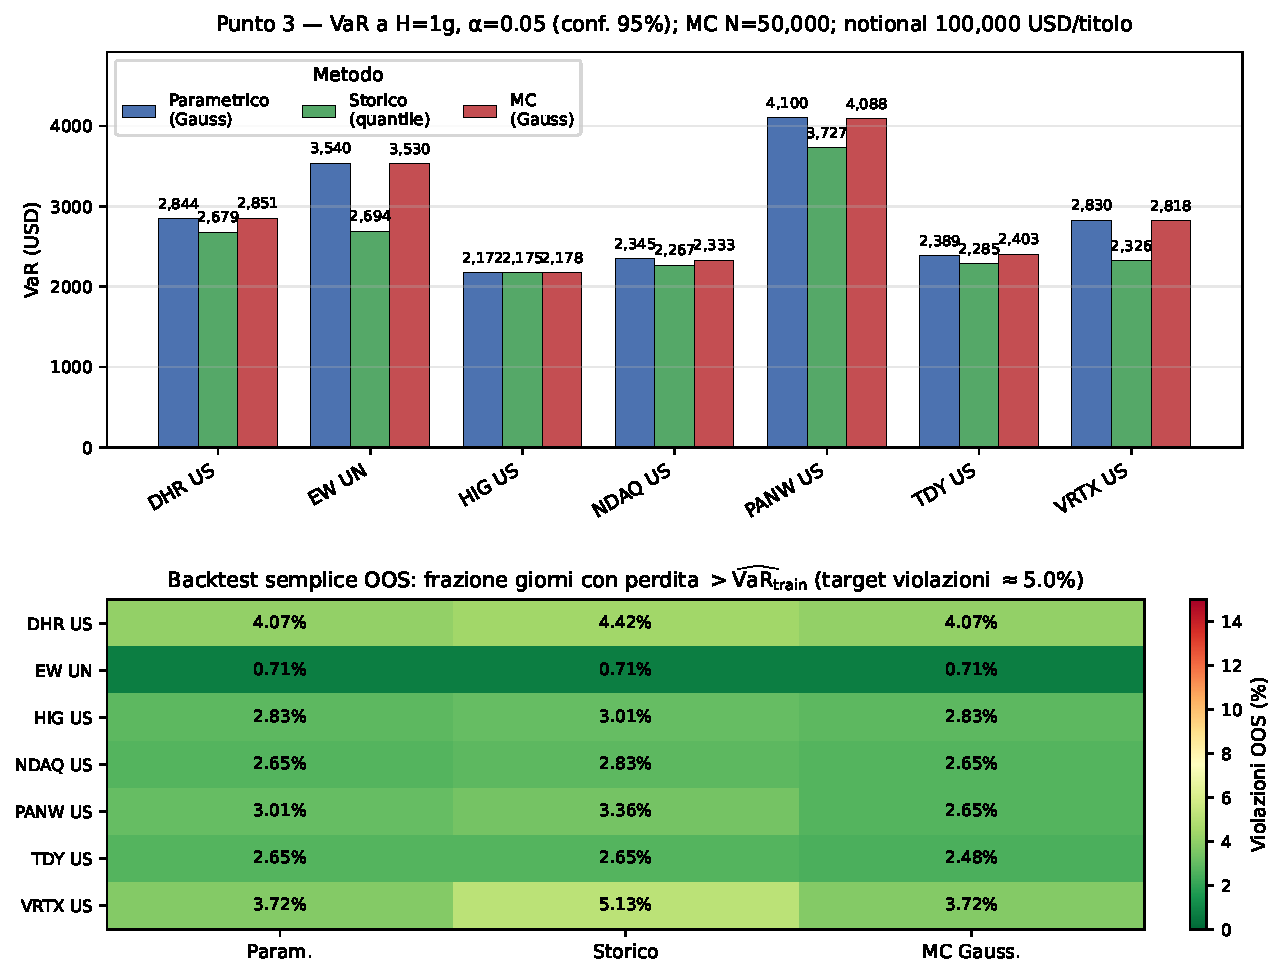
\includegraphics[width=0.88\textwidth]{p3_var_summary_and_oos_exceedance.pdf}
\caption{\VaR\ per metodo e violazioni OOS (target 5\%).}
\label{fig:p3_var}
\end{figure}

% =============================================================================
\section{Punto 4: Portafoglio con liquidità}
% =============================================================================

Pesi consegna: $90\%$ azioni (DHR, HIG, NDAQ, PANW, TDY $10\%$; EW, VRTX $20\%$) e $10\%$ liquidità a rendimento nullo. Analisi sugli \textbf{ultimi tre anni} (17/11/2022--17/11/2025): finestra richiesta dalla consegna e coerente con il profilo di rischio ``recente'' del portafoglio, senza diluire il triennio con osservazioni molto vecchie che appartengono a un regime di mercato diverso.

% -----------------------------------------------------------------------------
\subsection{Punto 4.a: Valore del portafoglio}
% -----------------------------------------------------------------------------

\subsubsection*{Costruzione di $V_t$ e implicazioni}

Il portafoglio segue un \textbf{buy-and-hold} senza ribilanciamento giornaliero:
\begin{equation}
  V_t = N\left(\sum_i w_i \frac{P_{i,t}}{P_{i,t_0}} + w_{\mathrm{cash}}\right),
  \qquad N=100\,000\USD,\quad w_{\mathrm{cash}}=10\%.
\end{equation}
La consegna fissa i pesi \emph{iniziali}; non ribilanciare significa che, se un titolo outperforma, il suo peso \emph{effettivo} nel portafoglio cresce nel tempo. \textbf{Vantaggio:} descrive un investitore che non ripristina i pesi ogni giorno. \textbf{Conseguenza metodologica:} il rendimento di portafoglio va definito come $g_{p,t}=\ln(V_t/V_{t-1})$ e non come $\sum_i w_i g_{i,t}$, altrimenti si ignora la deriva dei pesi e l'effetto della liquidità.

La quota di \textbf{liquidità al 10\%} ha rendimento nullo e volatilità nulla. Non entra in $\hat{\boldsymbol\Sigma}$ (varianza zero), ma riduce l'esposizione azionaria effettiva al 90\% del capitale: \textbf{implicazione} un \VaR\ di portafoglio più basso rispetto a un portafoglio fully invested sugli stessi titoli, a parità di matrice di covarianza azionaria.

\subsubsection*{Risultati e lettura della Figura~\ref{fig:p4a}}

Sul triennio 17/11/2022--17/11/2025 il total return semplice è $+41{,}58\%$ ($V_T\approx 141\,583\USD$). Prima della figura riassumiamo cosa leggere, così il grafico non resta scollegato dal testo.

\needspace{10\baselineskip}
\begin{figure}[htbp]
\centering
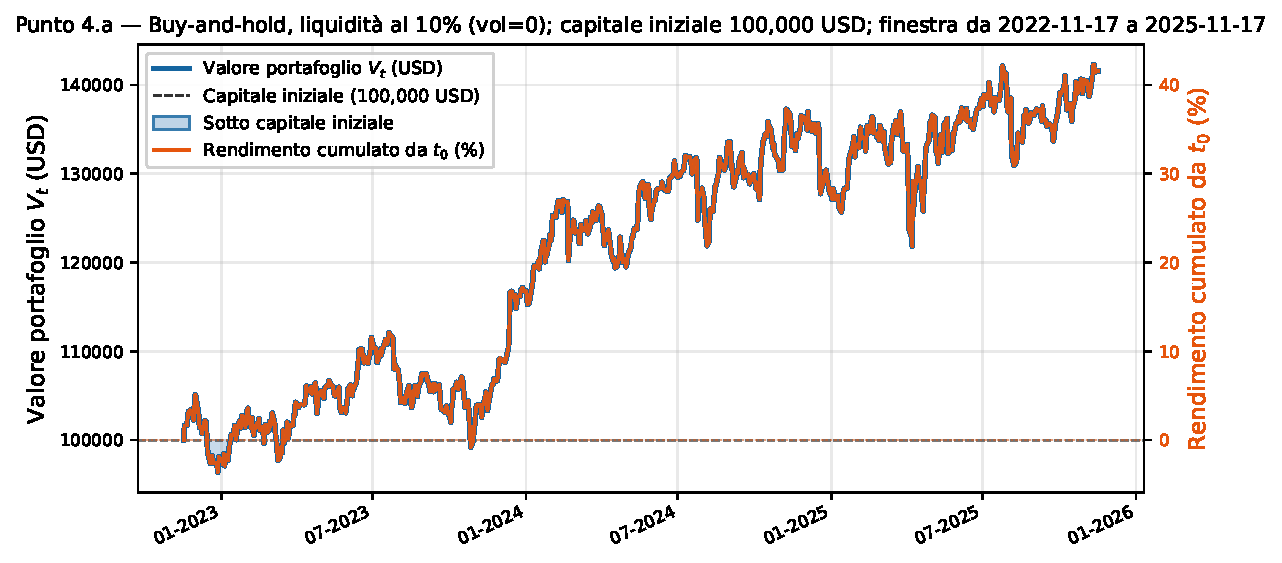
\includegraphics[width=0.88\textwidth]{p4a_portfolio_constant_weights_3y.pdf}
\caption{Valore del portafoglio $V_t$ (USD, linea blu) e rendimento cumulato da $t_0$ (asse destro, \%). Area azzurra: giorni con $V_t$ sotto i \$100\,000 iniziali.}
\label{fig:p4a}
\end{figure}
\FloatBarrier

La linea blu è $V_t$ in dollari; l'asse destro arancione è il rendimento cumulato percentuale da $t_0$. L'area sotto la linea tratteggiata dei \$100\,000 evidenzia le giornate in cui il portafoglio chiude in perdita rispetto al capitale iniziale: è un indicatore visivo di \emph{drawdown} rispetto al nominale, non il \VaR.

\textbf{Distinzione fondamentale rispetto al Punto~4.c.} Il \VaR\ al 5\% misura la perdita monetaria potenziale in \textbf{un solo giorno} peggiore (secondo il modello scelto), non la perdita massima osservata sul triennio né il drawdown cumulato. Un portafoglio può avere total return positivo (+41,58\%) e comunque giorni con $g_{p,t}$ molto negativi: il \VaR\ cattura proprio quel rischio di coda giornaliera. Confondere \VaR\ e drawdown massimo porterebbe a sottovalutare o sovravalutare il rischio operativo.

% -----------------------------------------------------------------------------
\subsection{Punto 4.b: Rendimenti e volatilità del portafoglio}
% -----------------------------------------------------------------------------

$g_{p,t}=\ln(V_t/V_{t-1})$ incorpora cash e non linearità. \textbf{Alternativa scartata:} $\sum w_i g_{i,t}$ sarebbe più semplice ma falserebbe il rischio quando i pesi effettivi driftano.

Vol rolling $21$ giorni, annualizzata $\sqrt{252}$: orizzonte di circa un mese di trading, standard nei report giornalieri (stesso ordine di grandezza dell'EWMA con $\lambda\approx 0{,}909$ al Punto~4.e). Su $782$ giorni: rendimento log $+34{,}77\%$, vol annua $15{,}18\%$. Fig.~\ref{fig:p4b}: cluster di $g_{p,t}$ negativi = stress; vol rolling sopra $15{,}18\%$ = regime più rischioso della media triennale.

\begin{figure}[H]
\centering
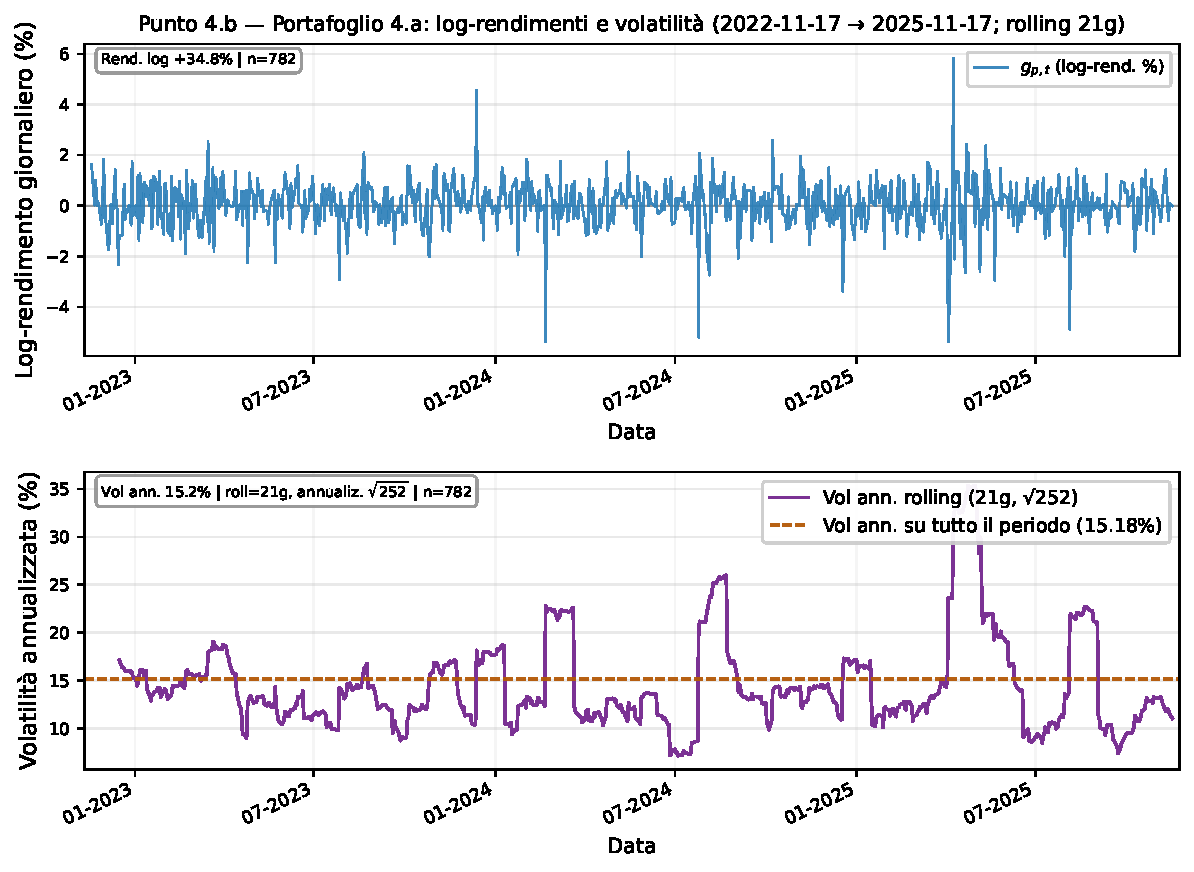
\includegraphics[width=0.88\textwidth]{p4b_portfolio_log_returns_and_rolling_vol.pdf}
\caption{$g_{p,t}$ e volatilità rolling 21g annualizzata.}
\label{fig:p4b}
\end{figure}

% -----------------------------------------------------------------------------
\subsection{Punto 4.c: VaR del portafoglio}
% -----------------------------------------------------------------------------

Stessi $\alpha=5\%$ e $H=1$ del Punto~3, ma $N=100\,000\USD$ \emph{unico} sul portafoglio. $\hat{\boldsymbol\Sigma}$ e $\hat\rho_{ij}$ sui rendimenti azionari dal $t_0$ del triennio ($n=783$ listwise); cash esclusa (varianza nulla).

\textbf{Parametrico (var-cov):} approssimazione $g_p\approx\mathbf{w}'\mathbf{g}$, $\hat\sigma_p=\sqrt{\mathbf{w}'\hat{\boldsymbol\Sigma}\mathbf{w}}$, $\VaR_g=-(\hat\mu_p+z_{0{,}05}\hat\sigma_p)$. \textbf{Vantaggio:} chiuso, veloce, usa tutta l'informazione lineare sulle coppie. \textbf{Limite:} ignora non linearità del buy-and-hold e code non gaussiane.

\textbf{Monte Carlo multivariato:} $50\,000$ vettori $\mathbf{g}\sim\mathcal{N}(\hat{\boldsymbol\mu},\hat{\boldsymbol\Sigma})$, quantile su $\mathbf{w}'\mathbf{g}$. Stessa $\hat{\boldsymbol\Sigma}$ del parametrico: verifica numerica. \textbf{Non} è simulazione di prezzi; \textbf{non} usa vol GARCH.

\textbf{Storico su $g_p$:} quantile empirico dei rendimenti reali del portafoglio. \textbf{Vantaggio:} unico metodo che rispetta cash e buy-and-hold senza imporre normalità. \textbf{Conseguenza osservata:} storico (\$1\,338) $<$ parametrico (\$1\,467): nel triennio le code empiriche del portafoglio sono state meno estreme della gaussiana con quella $\hat{\boldsymbol\Sigma}$.

Somma pesata \VaR\ marginali Punto~3 ($\approx\$2\,659$): \textbf{non} è \VaR\ di portafoglio (lì ogni titolo aveva \$100k separati). Fig.~\ref{fig:p4c}: barre a sinistra; heatmap $\hat\rho_{ij}$ a destra (NDAQ--TDY tra le più alte, $\hat\rho\approx 0{,}41$).

\begin{table}[H]
\centering
\footnotesize
\caption{\VaR\ portafoglio, $N=100\,000\USD$, $\alpha=5\%$, $H=1$g.}
\begin{tabular}{lrr}
\toprule
\textbf{Metodo} & \textbf{VaR log} & \textbf{VaR USD} \\
\midrule
Parametrico  & 0.01478 & 1{,}467 \\
Monte Carlo  & 0.01479 & 1{,}468 \\
Storico $g_p$& 0.01347 & 1{,}338 \\
\bottomrule
\end{tabular}
\end{table}

\begin{figure}[H]
\centering
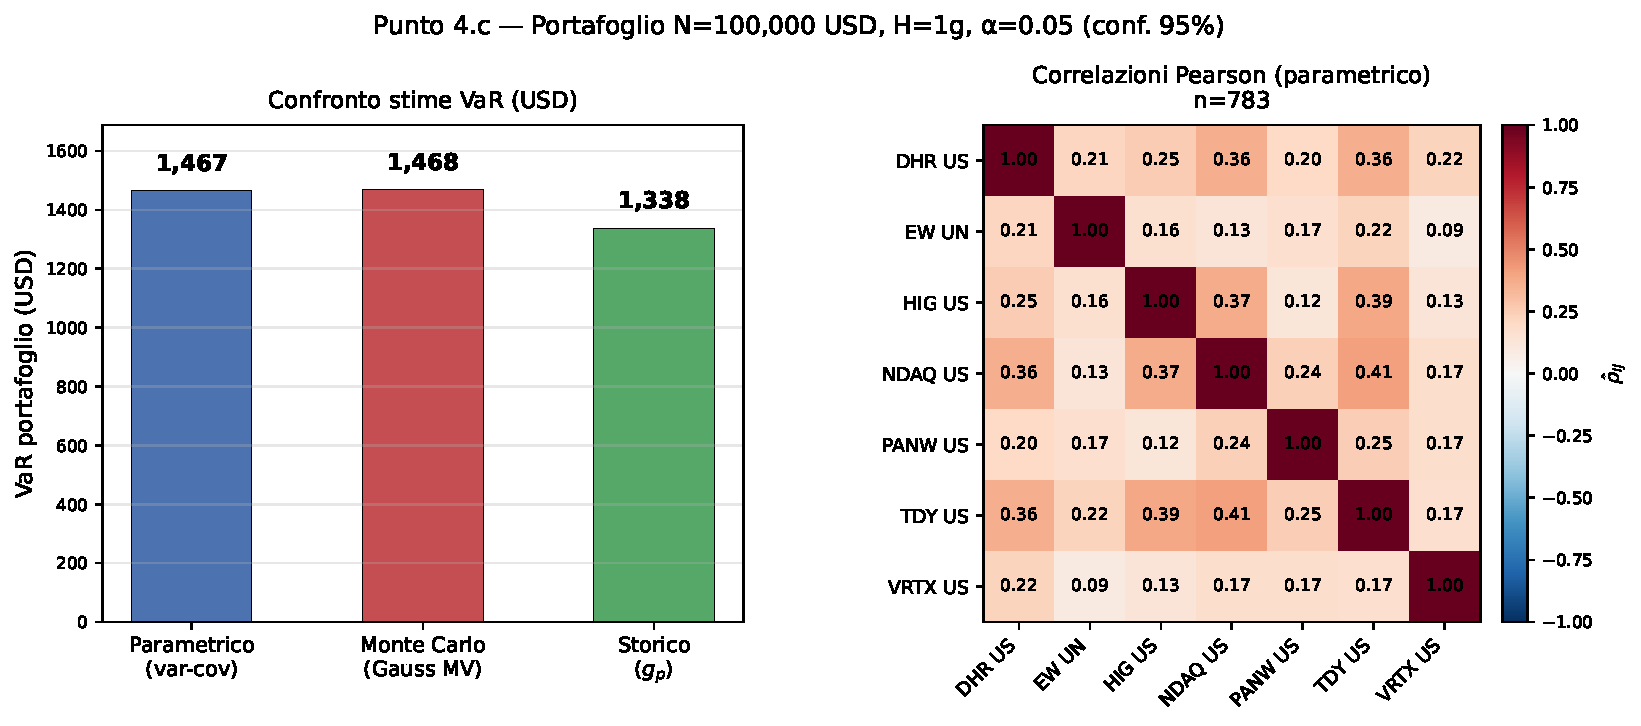
\includegraphics[width=0.88\textwidth]{p4c_portfolio_var_usd_and_correlations.pdf}
\caption{\VaR\ USD e $\hat\rho_{ij}$ del parametrico.}
\label{fig:p4c}
\end{figure}

% -----------------------------------------------------------------------------
\subsection{Punto 4.d: Diversificazione}
% -----------------------------------------------------------------------------

Confronto a tre scenari: $\hat{\boldsymbol\Sigma}$ piena (mondo reale); $\hat{\boldsymbol\Sigma}$ diagonale ($\rho_{ij}=0$, stesse vol marginali); storico su $g_p$. \textbf{Domanda economica:} quanto del rischio viene dalla vol dei singoli titoli e quanto dalla loro co-movimento?

Media $\hat\rho_{ij}\approx 0{,}23$; tutte le coppie significative al $5\%$. Correlazioni positive $\Rightarrow$ \VaR\ piena (\$1\,467) $>$ indipendenti (\$1\,057): le correlazioni \emph{aumentano} il rischio di circa \$410 ($+39\%$). \textbf{Interpretazione:} in stress i titoli US del campione tendono a scendere insieme; la diversificazione \emph{non} elimina il fattore mercato comune. Il portafoglio resta molto sotto \$2\,659 (somma ingenua dei \VaR\ titoli): il capitale unico e la covarianza riducono il rischio rispetto a quella somma, ma non rispetto allo scenario $\rho=0$.

Fig.~\ref{fig:p4d}: heatmap; barre parametrico pieno / diagonale / storico.

\begin{figure}[H]
\centering
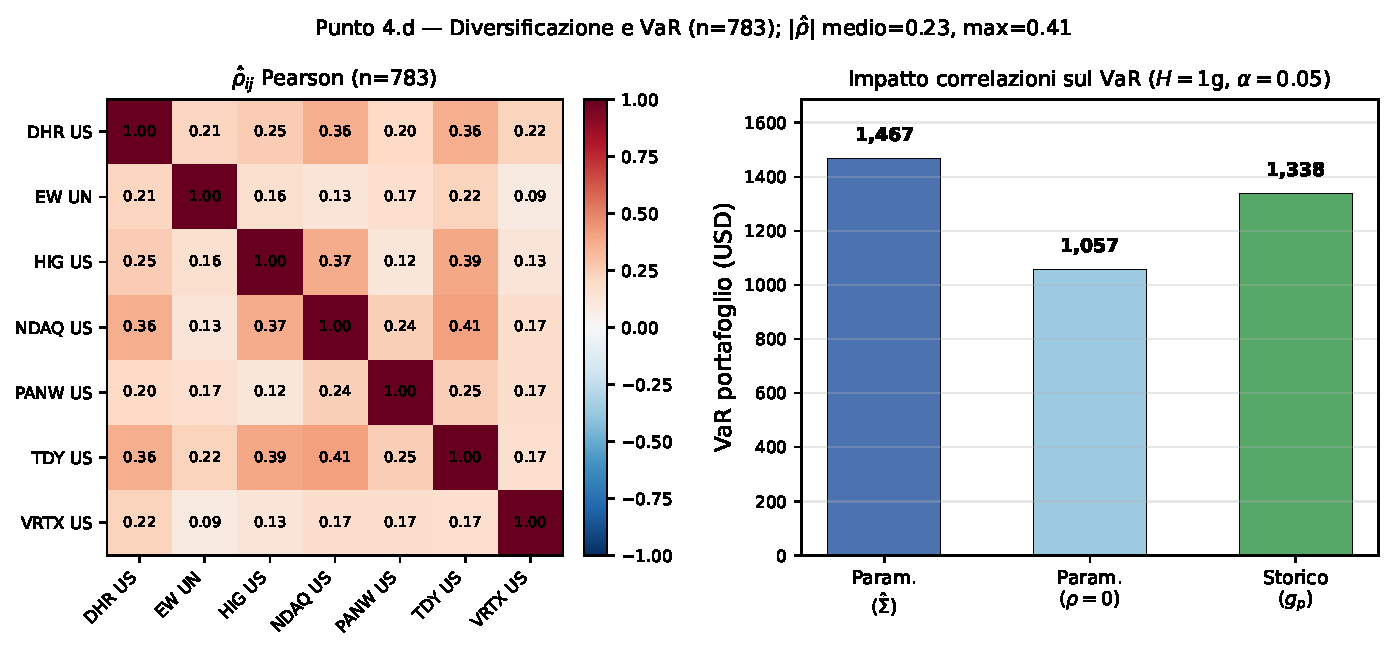
\includegraphics[width=0.88\textwidth]{p4d_diversification_correlations_and_var_impact.pdf}
\caption{$\hat\rho_{ij}$ e impatto sul \VaR.}
\label{fig:p4d}
\end{figure}

% -----------------------------------------------------------------------------
\subsection{Punto 4.e: La volatilità è costante?}
% -----------------------------------------------------------------------------

\textbf{Risposta: no.} Tre linee di evidenza su $g_{p,t}$.

\textbf{(i) Grafica.} Rolling 252g e 21g, EWMA ($\lambda\approx 0{,}909$), GARCH-$t$ ed EGARCH-$t$ (per asimmetria/leva se GARCH degenera). Se le curve si muovono nel tempo, l'ipotesi di vol costante è respinta visivamente.

\textbf{(ii) Sotto-periodi.} Vol annualizzata da $13{,}9\%$ (P1) a $15{,}0\%$ (P2) a $16{,}5\%$ (P3): drift crescente del rischio nel triennio.

\textbf{(iii) Test.} Bartlett ($p=0{,}023$): rigetta uguaglianza di varianze tra sotto-periodi (sensibile alla normalità). Levene ($p=0{,}51$): non rigetta; più robusto agli outlier, quindi la differenza di varianze non è guidata da pochi giorni estremi. ARCH-LM ($p\approx 4{,}3\times 10^{-4}$): forte evidenza di \textbf{eteroschedasticità condizionata} (effetto ARCH). Ljung--Box su $g_p^2$ (lag 20, $p=0{,}012$): autocorrelazione nei quadrati dei rendimenti, coerente con clustering.

Vol rolling 1Y: min $\approx 13{,}4\%$, max $\approx 17{,}6\%$ (rapporto $\approx 1{,}3$). \textbf{Conseguenza operativa:} un unico $\hat\sigma=15{,}18\%$ non basta per limiti di rischio dinamici; servono monitoraggio rolling o modelli condizionati.

Fig.~\ref{fig:p4e}: curve vs.\ benchmark $15{,}18\%$. Quando GARCH ed EWMA salgono insieme in fasi stressate (es.\ autunno 2022), l'ipotesi ``vol costante al 15,18\%'' è inaccettabile per limiti interni; quando scendono sotto la media, un unico numero statico \emph{sovrastimerebbe} il rischio corrente.

\needspace{8\baselineskip}
\begin{table}[htbp]
\centering
\footnotesize
\caption{Test su $g_{p,t}$ (triennio).}
\begin{tabular}{lrr}
\toprule
\textbf{Test} & \textbf{Stat.} & $p$ \\
\midrule
Bartlett (3 sotto-periodi) & 7,52 & 0,023 \\
Levene (3 sotto-periodi)   & 0,67 & 0,510 \\
ARCH-LM (10 lag)           & 31,84 & $4{,}3\times 10^{-4}$ \\
Ljung--Box $g_p^2$ (20)    & 36,93 & 0,012 \\
\bottomrule
\end{tabular}
\end{table}

\begin{figure}[H]
\centering
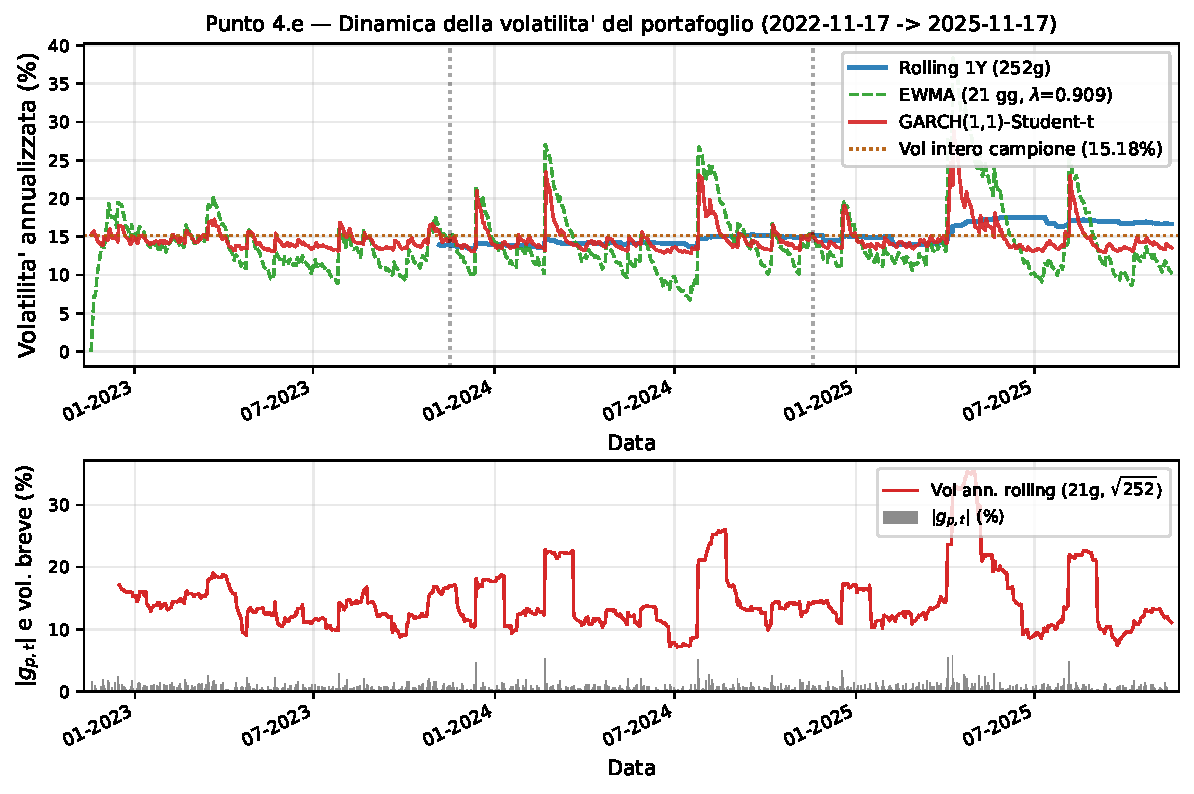
\includegraphics[width=0.88\textwidth]{p4e_portfolio_vol_dynamics.pdf}
\caption{Dinamiche di volatilità del portafoglio.}
\label{fig:p4e}
\end{figure}

% =============================================================================
\section{Quadro riepilogativo: parametri, modelli e implicazioni}
% =============================================================================

Questa sezione chiude il filo logico del report: ogni scelta numerica ha un motivo economico-statistico e una conseguenza sulla lettura dei risultati.

\textbf{Rendimenti e campione.} Log-rendimenti su prezzi USD: coerenza con GARCH e \VaR; rendimenti semplici solo per interpretare $V_t$. Campione lungo (Punti~1--3) vs.\ triennio (Punto~4): il \VaR\ di portafoglio usa il regime recente, dove correlazioni e vol possono differire dal lungo periodo.

\textbf{Volatilità.} Statica = benchmark storico unico. Rolling 21g/252g = regime attuale (1M/1Y). EWMA con $\lambda=0{,}94$: memoria lunga, adatta al monitoraggio giornaliero e al clustering; peso $(1-\lambda)=6\%$ sullo shock odierno, $(\lambda)=94\%$ sulla vol di ieri. EWMA con $\lambda\approx 0{,}909$ (equivalente 21g): più reattiva, allineata al mese di trading sul portafoglio. GARCH$(1,1)$-$t$: vol \emph{condizionata oggi}, cattura ARCH; Student-$t$ perché Jarque--Bera rigetta la normalità. EGARCH: leva e stime stabili se GARCH degenera. \textbf{Implicazione nel \VaR:} usiamo $\hat\sigma$ campionaria statica, non $\sigma_t^{\mathrm{GARCH}}$, così parametrico, storico e MC rispondono alla stessa domanda; GARCH/EWMA servono a dire \emph{se} e \emph{quando} quella vol media è fuorviante.

\textbf{Correlazioni.} Pearson listwise, test al 5\% (due code): standard industry; con $n$ grande attenzione alla magnitudine di $\hat\rho$, non solo al $p$-value. Matrice completa nel \VaR\ parametrico; scenario $\rho_{ij}=0$ nel Punto~4.d per quantificare l'effetto della co-movimentazione (+39\% di \VaR\ nel nostro campione).

\textbf{\VaR.} $\alpha=5\%$: compromesso stabilità/conservatività; stesso $\alpha$ su titoli e portafoglio per confrontabilità. $H=1$ giorno: consegna; scaling $\sqrt{H}$ solo come approssimazione gaussiana i.i.d. $M=100\,000\USD$: per titolo (Punto~3) vs.\ unico (Punto~4), interpretazioni diverse. Tre metodi: parametrico (ipotesi, velocità), storico (empirico, meno ipotesi), MC (verifica numerica del gaussiano). Cash 10\%: fuori da $\hat{\boldsymbol\Sigma}$, dentro $V_t$ e storico su $g_p$. Buy-and-hold: $g_p$ reale vs.\ $\mathbf{w}'\mathbf{g}$ nel gaussiano.

\textbf{Test Punto~4.e.} Bartlett: varianze diverse tra sotto-periodi. Levene: stessa conclusione robusta agli outlier. ARCH-LM e Ljung--Box su $g_p^2$: vol non costante, clustering. \textbf{Implicazione:} limiti di rischio dinamici, non un solo numero annuo.

% =============================================================================
\section{Conclusioni}
% =============================================================================

Il lavoro segue la consegna con un filo logico unico: definire bene le grandezze (log-rendimenti, $V_t$ buy-and-hold, $g_p$), misurare dispersione e dipendenza (vol statica/rolling/EWMA/GARCH, Pearson al 5\%), stimare il rischio con tre filosofie (\VaR\ parametrico, storico, MC) e verificarle incrociando numeri e grafici.

\textbf{Sintesi delle scelte chiave.} Log-rendimenti per coerenza temporale e con i modelli; $\lambda=0{,}94$ (titoli) vs.\ $\approx 0{,}909$ (portafoglio su 21g) per orizzonti diversi; GARCH/EGARCH per dinamica e leva, ma vol campionaria nel \VaR\ per confrontabilità; $\alpha=5\%$ sia sui test di correlazione sia sul \VaR; $H=1$ giorno; $M=100\,000\USD$ con interpretazione diversa tra Punto~3 (per titolo) e Punto~4 (portafoglio unico); cash 10\% fuori da $\hat{\boldsymbol\Sigma}$ ma dentro $V_t$ e lo storico su $g_p$.

\textbf{Risultati economici.} Parametrico e MC coincidono (implementazione e ipotesi gaussiana condivise); lo storico è spesso meno severo sul campione (code empiriche). Correlazioni positive alzano il \VaR\ rispetto al caso $\rho_{ij}=0$. La vol del portafoglio non è costante: monitoraggio dinamico necessario.

Tutte le cifre e le figure provengono dal notebook di gruppo, con parametri dichiarati in testa al file di calcolo e riproducibili.

\end{document}
